\documentclass[listof=totoc,index=totoc,bibliography=totoc,12pt,german,a4paper,]{report}
\usepackage{lmodern}

% use sans serif fonts
\renewcommand{\familydefault}{\sfdefault}

% german quote style, see:
% http://mirrors.ibiblio.org/CTAN/info/translations/csquotes/de/csquotes-DE.pdf
\usepackage[style = german]{csquotes}%

% Overwrite \begin{figure}[htbp] with \begin{figure}[H]
%\usepackage{float}
%\let\origfigure=\figure
%\let\endorigfigure=\endfigure
%\renewenvironment{figure}[1][]{%
%\origfigure[b]
%}{%
%\endorigfigure
%}

% fix for pandoc 1.14
\providecommand{\tightlist}{%
  \setlength{\itemsep}{0pt}\setlength{\parskip}{0pt}}

% TP: hack to truncate list of figures/tables.
\usepackage{truncate}
\usepackage{caption}
\usepackage{tocloft}
% TP: end hack

\usepackage{amssymb,amsmath}
\usepackage{ifxetex,ifluatex}

% Only use fixltx2e if using pre-2015 kernels
\begingroup\expandafter\expandafter\expandafter\endgroup
\expandafter\ifx\csname IncludeInRelease\endcsname\relax
  \usepackage{fixltx2e}
\fi

\ifnum 0\ifxetex 1\fi\ifluatex 1\fi=0 % if pdftex
  \usepackage[T1]{fontenc}
  \usepackage[utf8]{inputenc}
\mathbf{
\else % if luatex or xelatex
  \ifxetex
    \usepackage{mathspec}
    \usepackage{xltxtra,xunicode}
  \else
    \usepackage{fontspec}
  \fi
  \defaultfontfeatures{Mapping=tex-text,Scale=MatchLowercase}
  \newcommand{\euro}{€}
\fi
% use upquote if available, for straight quotes in verbatim environments
\IfFileExists{upquote.sty}{\usepackage{upquote}}{}
% use microtype if available
\IfFileExists{microtype.sty}{%
\usepackage{microtype}
\UseMicrotypeSet[protrusion]{basicmath} % disable protrusion for tt fonts
}{}
\usepackage{color}
\usepackage{fancyvrb}
\newcommand{\VerbBar}{|}
\newcommand{\VERB}{\Verb[commandchars=\\\{\}]}
\DefineVerbatimEnvironment{Highlighting}{Verbatim}{commandchars=\\\{\}}
% Add ',fontsize=\small' for more characters per line
\newenvironment{Shaded}{}{}
\newcommand{\AlertTok}[1]{\textcolor[rgb]{1.00,0.00,0.00}{\textbf{#1}}}
\newcommand{\AnnotationTok}[1]{\textcolor[rgb]{0.38,0.63,0.69}{\textbf{\textit{#1}}}}
\newcommand{\AttributeTok}[1]{\textcolor[rgb]{0.49,0.56,0.16}{#1}}
\newcommand{\BaseNTok}[1]{\textcolor[rgb]{0.25,0.63,0.44}{#1}}
\newcommand{\BuiltInTok}[1]{\textcolor[rgb]{0.00,0.50,0.00}{#1}}
\newcommand{\CharTok}[1]{\textcolor[rgb]{0.25,0.44,0.63}{#1}}
\newcommand{\CommentTok}[1]{\textcolor[rgb]{0.38,0.63,0.69}{\textit{#1}}}
\newcommand{\CommentVarTok}[1]{\textcolor[rgb]{0.38,0.63,0.69}{\textbf{\textit{#1}}}}
\newcommand{\ConstantTok}[1]{\textcolor[rgb]{0.53,0.00,0.00}{#1}}
\newcommand{\ControlFlowTok}[1]{\textcolor[rgb]{0.00,0.44,0.13}{\textbf{#1}}}
\newcommand{\DataTypeTok}[1]{\textcolor[rgb]{0.56,0.13,0.00}{#1}}
\newcommand{\DecValTok}[1]{\textcolor[rgb]{0.25,0.63,0.44}{#1}}
\newcommand{\DocumentationTok}[1]{\textcolor[rgb]{0.73,0.13,0.13}{\textit{#1}}}
\newcommand{\ErrorTok}[1]{\textcolor[rgb]{1.00,0.00,0.00}{\textbf{#1}}}
\newcommand{\ExtensionTok}[1]{#1}
\newcommand{\FloatTok}[1]{\textcolor[rgb]{0.25,0.63,0.44}{#1}}
\newcommand{\FunctionTok}[1]{\textcolor[rgb]{0.02,0.16,0.49}{#1}}
\newcommand{\ImportTok}[1]{\textcolor[rgb]{0.00,0.50,0.00}{\textbf{#1}}}
\newcommand{\InformationTok}[1]{\textcolor[rgb]{0.38,0.63,0.69}{\textbf{\textit{#1}}}}
\newcommand{\KeywordTok}[1]{\textcolor[rgb]{0.00,0.44,0.13}{\textbf{#1}}}
\newcommand{\NormalTok}[1]{#1}
\newcommand{\OperatorTok}[1]{\textcolor[rgb]{0.40,0.40,0.40}{#1}}
\newcommand{\OtherTok}[1]{\textcolor[rgb]{0.00,0.44,0.13}{#1}}
\newcommand{\PreprocessorTok}[1]{\textcolor[rgb]{0.74,0.48,0.00}{#1}}
\newcommand{\RegionMarkerTok}[1]{#1}
\newcommand{\SpecialCharTok}[1]{\textcolor[rgb]{0.25,0.44,0.63}{#1}}
\newcommand{\SpecialStringTok}[1]{\textcolor[rgb]{0.73,0.40,0.53}{#1}}
\newcommand{\StringTok}[1]{\textcolor[rgb]{0.25,0.44,0.63}{#1}}
\newcommand{\VariableTok}[1]{\textcolor[rgb]{0.10,0.09,0.49}{#1}}
\newcommand{\VerbatimStringTok}[1]{\textcolor[rgb]{0.25,0.44,0.63}{#1}}
\newcommand{\WarningTok}[1]{\textcolor[rgb]{0.38,0.63,0.69}{\textbf{\textit{#1}}}}
\usepackage{longtable,booktabs}
\usepackage{graphicx}
\makeatletter
\def\maxwidth{\ifdim\Gin@nat@width>\linewidth\linewidth\else\Gin@nat@width\fi}
\def\maxheight{\ifdim\Gin@nat@height>\textheight\textheight\else\Gin@nat@height\fi}
\makeatother
% Scale images if necessary, so that they will not overflow the page
% margins by default, and it is still possible to overwrite the defaults
% using explicit options in \includegraphics[width, height, ...]{}
\setkeys{Gin}{width=\maxwidth,height=\maxheight,keepaspectratio}

\setlength{\parindent}{0pt}
\setlength{\parskip}{6pt plus 2pt minus 1pt}
\setlength{\emergencystretch}{3em}  % prevent overfull lines
\setcounter{secnumdepth}{5}
\ifxetex
  \usepackage{polyglossia}
  \setmainlanguage{german}
\else
  \usepackage[german]{babel}
\fi

% % \newlength{\cslhangindent}
% \setlength{\cslhangindent}{1.5em}
% \newenvironment{cslreferences}%
%   {}%
%   {\par}
% 
\newlength{\cslhangindent}
\setlength{\cslhangindent}{1.5em}
\newlength{\csllabelwidth}
\setlength{\csllabelwidth}{3em}
\newenvironment{CSLReferences}[2] % #1 hanging-ident, #2 entry spacing
 {% don't indent paragraphs
  \setlength{\parindent}{0pt}
  % turn on hanging indent if param 1 is 1
  \ifodd #1 \everypar{\setlength{\hangindent}{\cslhangindent}}\ignorespaces\fi
  % set entry spacing
  \ifnum #2 > 0
  \setlength{\parskip}{#2\baselineskip}
  \fi
 }%
 {}
\usepackage{calc}
\newcommand{\CSLBlock}[1]{#1\hfill\break}
\newcommand{\CSLLeftMargin}[1]{\parbox[t]{\csllabelwidth}{#1}}
\newcommand{\CSLRightInline}[1]{\parbox[t]{\linewidth - \csllabelwidth}{#1}\break}
\newcommand{\CSLIndent}[1]{\hspace{\cslhangindent}#1}

% Table of contents formatting
\renewcommand{\contentsname}{Table of Contents}
\setcounter{tocdepth}{3}

% Number of the last page in the document
\usepackage{lastpage}

% Set margins
% HAS TO BE before the \usepackage{fancyhdr} and \pagestyle{fancy} commands
% Otherwise header and footer line will not match textwidth.
\usepackage[top=2.5cm,bottom=2.5cm,left=3.5cm,right=2.5cm]{geometry}
%\setlength\parindent{0.4in} % indent at start of paragraphs (set to 0.3?)

% Headers and page numbering
\usepackage{fancyhdr}
\pagestyle{fancy}
\fancyhf{}
\rhead{\rightmark}
%\rfoot{\thepage\space von \pageref{LastPage}}
\rfoot{\thepage}
\renewcommand{\headrulewidth}{0.5pt}
\renewcommand{\footrulewidth}{0.5pt}
%\setlength\voffset{0.2cm}

% Following package is used to add background image to front page
\usepackage{wallpaper}

% Table package
\usepackage{ctable}% http://ctan.org/pkg/ctable

% Deal with 'LaTeX Error: Too many unprocessed floats.'
\usepackage{morefloats}
% or use \extrafloats{100}
% add some \clearpage

% % Chapter header
\usepackage{titlesec, blindtext, color}
\definecolor{gray75}{gray}{0.75}
\newcommand{\hsp}{\hspace{20pt}}
\titleformat{\chapter}[hang]{\Huge\bfseries}{\thechapter\hsp\textcolor{gray75}{|}\hsp}{0pt}{\Huge\bfseries}

% How should the first page of a chapter be handled? e.g. page number 
% https://tex.stackexchange.com/a/10044
%\makeatletter
%\renewcommand\chapter{\if@openright\cleardoublepage\else\clearpage\fi
%                    \thispagestyle{fancy}%
%                    \global\@topnum\z@
%                    \@afterindentfalse
%                    \secdef\@chapter\@schapter}
%\makeatother{}

%Redefine plain for first chapter site
\fancypagestyle{plain}{%
\fancyhf{}%
\fancyfoot[R]{\thepage}%
\renewcommand{\headrulewidth}{0.0pt}%
\renewcommand{\footrulewidth}{0.0pt}%
}

% FONTS
\usepackage{xunicode}
\usepackage{xltxtra}
\defaultfontfeatures{Mapping=tex-text} % converts LaTeX specials (``quotes'' --- dashes etc.) to unicode

% CODE BLOCKS
\usepackage[utf8]{inputenc}
\usepackage{listings}
\usepackage{color}

% JAVA CODE BLOCKS
\definecolor{backcolour}{RGB}{242,242,242}
\definecolor{javared}{rgb}{0.6,0,0}
\definecolor{javagreen}{rgb}{0.25,0.5,0.35}
\definecolor{javapurple}{rgb}{0.5,0,0.35}
\definecolor{javadocblue}{rgb}{0.25,0.35,0.75}

\lstdefinestyle{javaCodeStyle}{
  language=Java,                         % the language of the code
  backgroundcolor=\color{backcolour},    % choose the background color; you must add \usepackage{color} or \usepackage{xcolor}
  basicstyle=\fontsize{10}{8}\sffamily,
  breakatwhitespace=false,
  breaklines=true,
  keywordstyle=\color{javapurple}\bfseries,
  stringstyle=\color{javared},
  commentstyle=\color{javagreen},
  morecomment=[s][\color{javadocblue}]{/**}{*/},
  captionpos=t,                          % sets the caption-position to bottom
  frame=single,                          % adds a frame around the code
  numbers=left,
  numbersep=10pt,                         % margin between number and code block
  keepspaces=true,                       % keeps spaces in text, useful for keeping indentation of code (possibly needs columns=flexible)
  columns=fullflexible,
  showspaces=false,                      % show spaces everywhere adding particular underscores; it overrides 'showstringspaces'
  showstringspaces=false,                % underline spaces within strings only
  showtabs=false,                        % show tabs within strings adding particular underscores
  tabsize=2                              % sets default tabsize to 2 spaces
}

%Attempt to set math size
%First size must match the text size in the document or command will not work
%\DeclareMathSizes{display size}{text size}{script size}{scriptscript size}.
%\DeclareMathSizes{12}{13}{7}{7}

% Set figure legends and captions to be smaller sized sans serif font
\usepackage[font={footnotesize,sf}]{caption}
\captionsetup[table]{position=bottom}

\usepackage{siunitx}

% Adjust spacing between lines to 1.5
\usepackage{setspace}
% \onehalfspacing
\doublespacing
\raggedbottom

% Add space between pararaphs
% http://texblog.org/2012/11/07/correctly-typesetting-paragraphs-in-latex/
\setlength{\parskip}{8pt}

% Tables
\usepackage{booktabs}
\usepackage{threeparttable}
\usepackage{array}
\usepackage{makecell}
\newcolumntype{x}[1]{%
>{\centering\arraybackslash}m{#1}}%

% Allow for long captions and float captions on opposite page of figures
% \usepackage[rightFloats, CaptionBefore]{fltpage}

% Don't let floats cross subsections
% \usepackage[section,subsection]{extraplaceins}

% Rotate images and tables
\usepackage{float}
\usepackage{pdfpages}
\usepackage{pdflscape}
\usepackage{graphicx}
\usepackage{rotating}

% Custom math
\usepackage{bbold}
\DeclareMathOperator*{\argmin}{\arg\!\min}

% pandoc-crossref definitions

% We add the lines below from pandoc-crossref because we are using the --include-in-header flag
% see here: https://lierdakil.github.io/pandoc-crossref/#latex-output-and---include-in-header
% This LaTeX code is obtained by getting pandoc-crossref to dump it
% see here: https://github.com/lierdakil/pandoc-crossref/issues/326

\makeatletter
\@ifpackageloaded{subfig}{}{\usepackage{subfig}}
\@ifpackageloaded{caption}{}{\usepackage{caption}}
\captionsetup[subfloat]{margin=0.5em}
\AtBeginDocument{%
\renewcommand*\figurename{Figure}
\renewcommand*\tablename{Table}
}
\AtBeginDocument{%
\renewcommand*\listfigurename{List of Figures}
\renewcommand*\listtablename{List of Tables}
}
\newcounter{pandoccrossref@subfigures@footnote@counter}
\newenvironment{pandoccrossrefsubfigures}{%
\setcounter{pandoccrossref@subfigures@footnote@counter}{0}
\begin{figure}\centering%
\gdef\global@pandoccrossref@subfigures@footnotes{}%
\DeclareRobustCommand{\footnote}[1]{\footnotemark%
\stepcounter{pandoccrossref@subfigures@footnote@counter}%
\ifx\global@pandoccrossref@subfigures@footnotes\empty%
\gdef\global@pandoccrossref@subfigures@footnotes{{##1}}%
\else%
\g@addto@macro\global@pandoccrossref@subfigures@footnotes{, {##1}}%
\fi}}%
{\end{figure}%
\addtocounter{footnote}{-\value{pandoccrossref@subfigures@footnote@counter}}
\@for\f:=\global@pandoccrossref@subfigures@footnotes\do{\stepcounter{footnote}\footnotetext{\f}}%
\gdef\global@pandoccrossref@subfigures@footnotes{}}
\@ifpackageloaded{float}{}{\usepackage{float}}
\floatstyle{ruled}
\@ifundefined{c@chapter}{\newfloat{codelisting}{h}{lop}}{\newfloat{codelisting}{h}{lop}[chapter]}
\floatname{codelisting}{Listing}
\newcommand*\listoflistings{\listof{codelisting}{List of Listings}}
\makeatother

% References; This whole block should be the last before \begin{document}
\usepackage[hyphens]{url} % enables line breaks in urls at hyphens
\ifxetex
  \usepackage[setpagesize=false, % page size defined by xetex
              unicode=false, % unicode breaks when used with xetex
              xetex]{hyperref}
\else
  \usepackage[unicode=true]{hyperref}
\fi
\hypersetup{breaklinks=true,
            bookmarks=true,
            pdfauthor={Firstname Surname},
            pdftitle={This is the title of the thesis},
            colorlinks=false,
            citecolor=blue,
            urlcolor=blue,
            linkcolor=black,
            linktoc=section}
\urlstyle{same}  % don't use monospace font for urls
\usepackage[figure]{hypcap}

\begin{document}


% This is where the converted markdown files will go 
\% Abschlussarbeit \newcommand{\titel}{Titel der Abschlussarbeit}
\newcommand{\titelEN}{Title of your thesis}
\newcommand{\datum}{01.03.2018}

\% Autor\_in \newcommand{\aVorname}{Max}
\newcommand{\aNachname}{Mustermann}
\newcommand{\aGeburtsdatum}{01.04.1998}
\newcommand{\aInstitution}{Hochschule München}
\newcommand{\aStudiengruppe}{IF7} \newcommand{\aSemester}{WS 17/2018}
\newcommand{\aMatrikelnummer}{12345678}

\newcommand{\aName}{\aVorname\space\aNachname}

\% Prüfer\_in \newcommand{\pTitle}{Prof. Dr.} \newcommand{\pVorname}{}
\newcommand{\pNachname}{} \newcommand{\pInstitution}{Hochschule München}

\% Betreuer\_in \newcommand{\bTitle}{Dr.} \newcommand{\bVorname}{}
\newcommand{\bNachname}{} \newcommand{\bInstitution}{Firma GmbH}

\title{Titel der Abschlussarbeit}
\author{Max\space Mustermann}

\begin{titlepage}
    \begin{center}
        
\includegraphics[width=1\textwidth]{style/hm-fk07_logo.jpg}

        \Large
        Titel der Abschlussarbeit
        
        \normalsize
        Title of your thesis

        \vspace{0.5cm}
        \Large
        Max\space Mustermann

        \normalsize
        Bachelorarbeit Informatik

        \vfill

        \normalsize
        Prüfer:\\
        Prof. Dr.\space\space,\space Hochschule München

        % Firmenlogo
        % \includegraphics[width=0.4\textwidth]{style/firmenlogo.png}

        \normalsize
        Betreuer:\\
        Dr.\space\space,\space Firma GmbH

        % Abgabedatum
        01.03.2018

    \end{center}
\end{titlepage}

\chapter*{Erklärung}\label{erkluxe4rung}
\addcontentsline{toc}{chapter}{Erklärung}

\begin{center}
  Max\space Mustermann, geb. 01.04.1998\space(IF7,\space WS 17/2018, Matrikelnummer: 12345678)
\end{center}

\vspace*{1.0cm}

\noindent Hiermit erkläre ich, dass ich die Bachelorarbeit selbständig
verfasst, noch nicht anderweitig für Prüfungszwecke vorgelegt, keine
anderen als die angegebenen Quellen oder Hilfsmittel benutzt sowie
wörtliche und sinngemäße Zitate als solche gekennzeichnet habe.

\vspace*{1.0cm}

München, 01.03.2018

\vspace*{1.0cm}

\dotfill

Unterschrift \vspace*{\fill} \pagenumbering{gobble} \newpage

\chapter*{Abstract}\label{abstract}
\addcontentsline{toc}{chapter}{Abstract}

Lorem ipsum dolor sit amet, consectetur adipiscing elit. Nam et turpis
gravida, lacinia ante sit amet, sollicitudin erat. Aliquam efficitur
vehicula leo sed condimentum. Phasellus lobortis eros vitae rutrum
egestas. Vestibulum ante ipsum primis in faucibus orci luctus et
ultrices posuere cubilia Curae; Donec at urna imperdiet, vulputate orci
eu, sollicitudin leo. Donec nec dui sagittis, malesuada erat eget,
vulputate tellus. Nam ullamcorper efficitur iaculis. Mauris eu vehicula
nibh. In lectus turpis, tempor at felis a, egestas fermentum massa.

\pagenumbering{roman}
\setcounter{page}{1}

\newpage

\chapter*{Danksagungen}\label{danksagungen}
\addcontentsline{toc}{chapter}{Danksagungen}

Interdum et malesuada fames ac ante ipsum primis in faucibus. Aliquam
congue fermentum ante, semper porta nisl consectetur ut. Duis ornare sit
amet dui ac faucibus. Phasellus ullamcorper leo vitae arcu ultricies
cursus. Duis tristique lacus eget metus bibendum, at dapibus ante
malesuada. In dictum nulla nec porta varius. Fusce et elit eget sapien
fringilla maximus in sit amet dui.

Mauris eget blandit nisi, faucibus imperdiet odio. Suspendisse blandit
dolor sed tellus venenatis, venenatis fringilla turpis pretium. Donec
pharetra arcu vitae euismod tincidunt. Morbi ut turpis volutpat,
ultrices felis non, finibus justo. Proin convallis accumsan sem ac
vulputate. Sed rhoncus ipsum eu urna placerat, sed rhoncus erat
facilisis. Praesent vitae vestibulum dui. Proin interdum tellus ac velit
varius, sed finibus turpis placerat.

\pagenumbering{roman}
\setcounter{page}{2}

\newpage

\pagenumbering{gobble}

\rhead{}

\setcounter{tocdepth}{2}

\tableofcontents

\newpage

\pagenumbering{arabic}

\rhead{\rightmark}

\chapter*{Abbildungsverzeichnis}\label{abbildungsverzeichnis}
\addcontentsline{toc}{chapter}{Abbildungsverzeichnis}

\renewcommand{\listfigurename}{}

\listoffigures

\pagenumbering{roman}
\setcounter{page}{3}
\newpage

\chapter*{Tabellenverzeichnis}\label{tabellenverzeichnis}
\addcontentsline{toc}{chapter}{Tabellenverzeichnis}

\renewcommand{\listtablename}{}

\listoftables

\newpage

\chapter*{Abkürzungsverzeichnis}\label{abkuxfcrzungsverzeichnis}
\addcontentsline{toc}{chapter}{Abkürzungsverzeichnis}

\section*{Nicht ausgerichtet}\label{nicht-ausgerichtet}
\addcontentsline{toc}{section}{Nicht ausgerichtet}

API: \textbf{A}pplication \textbf{P}rogramming \textbf{I}nterface

JSON: \textbf{J}ava\textbf{S}cript \textbf{O}bject \textbf{N}otation

\section*{Ausgerichtet}\label{ausgerichtet}
\addcontentsline{toc}{section}{Ausgerichtet}

\begin{tabbing}
\textbf{API}~~~~~~~~~~~~ \= \textbf{A}pplication \textbf{P}rogramming \textbf{I}nterface \\  
\textbf{JSON} \> \textbf{J}ava\textbf{S}cript \textbf{O}bject \textbf{N}otation \\  
\end{tabbing}

\newpage

\setcounter{page}{1}
\pagenumbering{arabic}
\doublespacing
\setlength{\parindent}{0.5in}

\chapter{Einleitung mit Zitat}\label{sec:intro}

\section{Hintergrund}\label{hintergrund}

Das ist die Einleitung. Quisque finibus aliquet cursus. Integer in
pellentesque tellus. Duis eu dignissim nulla, a porttitor enim. Quisque
vehicula leo non ultrices finibus. Duis vehicula quis sem sit amet
sollicitudin. Integer neque est, pharetra et auctor vel, iaculis
interdum lectus.

Um ein Zitat in den Text aufzunehmen, füge einfach den in der
references.bib-Datei gezeigten Zitatschlüssel hinzu. Der Stil des Zitats
wird durch die Datei ref\_format.csl bestimmt. Zum Beispiel findest Du
in \emph{The Living Sea} Bilder vom \emph{Calypso} {[}1{]}.

In neque mauris, maximus at sapien a, iaculis dignissim justo. Aliquam
erat volutpat. Praesent varius risus auctor est ultricies, sit amet
consequat nisi laoreet. Suspendisse non est et mauris pharetra sagittis
non porta justo. Praesent malesuada metus ut sapien sodales ornare.

\section{Der Mittelteil}\label{der-mittelteil}

Das ist der Mittelteil. Phasellus quis ex in ipsum pellentesque lobortis
tincidunt sed massa. Nullam euismod sem quis dictum condimentum.
Suspendisse risus metus, elementum eu congue quis, viverra ac metus.
Donec non lectus at lectus euismod laoreet pharetra semper dui. Donec
sed eleifend erat, vel ultrices nibh. Nam scelerisque turpis ac nunc
mollis, et rutrum nisl luctus.

Duis faucibus vestibulum elit, sit amet lobortis libero. Class aptent
taciti sociosqu ad litora torquent per conubia nostra, per inceptos
himenaeos. Sed at cursus nibh. Sed accumsan imperdiet interdum. Proin id
facilisis tortor. Proin posuere a neque nec iaculis. Suspendisse
potenti. Nullam hendrerit ante mi, vitae iaculis dui laoreet eu.

Cras eleifend velit diam, eu viverra mi volutpat ut. Cum sociis natoque
penatibus et magnis dis parturient montes, nascetur ridiculus mus. Donec
finibus leo nec dui imperdiet, tincidunt ornare orci venenatis. Maecenas
placerat efficitur est, eu blandit magna hendrerit eu.

\subsection{Unterabschnitt des
Mittelteils}\label{unterabschnitt-des-mittelteils}

Das ist ein Unterabschnitt des Mittelteils. Quisque sit amet tempus
arcu, ac suscipit ante. Cras massa elit, pellentesque eget nisl ut,
malesuada rutrum risus. Nunc in venenatis mi. Curabitur sit amet
suscipit eros, non tincidunt nibh. Phasellus lorem lectus, iaculis non
luctus eget, tempus non risus. Suspendisse ut felis mi.

\section{Zusammenfassung der Kapitel}\label{zusammenfassung-der-kapitel}

Dies ist ein kurzer Überblick darüber, was in jedem Kapitel geschrieben
wurde. \textbf{Kapitel 1} gibt einen Hintergrund über duis tempus justo
quis arcu consectetur sollicitudin. \textbf{Kapitel 2} diskutiert morbi
sollicitudin gravida tellus in maximus. \textbf{Kapitel 3} diskutiert
vestibulum eleifend turpis id turpis sollicitudin aliquet.
\textbf{Kapitel 4} zeigt wie phasellus gravida non ex id aliquet. Proin
faucibus nibh sit amet augue blandit varius.

\chapter{Literaturübersicht mit Mathe}\label{sec:lit-review}

\section{Einleitung}\label{einleitung}

Das ist die Einleitung. Duis in neque felis. In hac habitasse platea
dictumst. Cras eget rutrum elit. Pellentesque tristique venenatis
pellentesque. Cras eu dignissim quam, vel sodales felis. Vestibulum
efficitur justo a nibh cursus eleifend. Integer ultrices lorem at nunc
efficitur lobortis.

\section{Der Mittelteil}\label{der-mittelteil-1}

Das ist die Literaturübersicht. Nullam quam odio, volutpat ac ornare
quis, vestibulum nec nulla. Aenean nec dapibus in
mL/min\textsuperscript{-1}. Mathematical formula can be inserted using
Latex:

\begin{equation}\protect\hypertarget{eq:my_equation}{}{f(x) = ax^3 + bx^2 + cx + d}\label{eq:my_equation}\end{equation}

Nunc eleifend, ex a luctus porttitor, felis ex suscipit tellus, ut
sollicitudin sapien purus in libero. Nulla blandit eget urna vel tempus.
Praesent fringilla dui sapien, sit amet egestas leo sollicitudin at.

Later on in the text, you can reference Equation~\ref{eq:my_equation}
and its mind-blowing ramifications. Pellentesque habitant morbi
tristique senectus et netus et malesuada fames ac turpis egestas. Sed
faucibus pulvinar volutpat. Ut semper fringilla erat non dapibus. Nunc
vitae felis eget purus placerat finibus laoreet ut nibh.

\section{A complicated math equation}\label{a-complicated-math-equation}

The following raw text in markdown behind
Equation~\ref{eq:my_complicated_equation} shows that you can fall back
on \LaTeX if it is more convenient for you. Note that this will only be
rendered in \texttt{thesis.pdf}

\begin{equation}\protect\hypertarget{eq:my_complicated_equation}{}{
\begin{aligned}
    \hat{\theta}_g = \argmin_{\theta_g} \Big\{ - &\sum^{N}_{n=1}\Big( 1-\mathbb{1}[f(\pmb x^{(n)})]\Big)\log f\Big(\pmb x^{(n)} \\ 
    &+ g(\pmb x^{(n)};\theta_g)\Big) + \lambda|g(\pmb x^{(n)};\theta_g)|_2 \Big\} \ ,
\end{aligned}
}\label{eq:my_complicated_equation}\end{equation}

\section{Fazit}\label{fazit}

Das ist das Fazit. Donec pulvinar molestie urna eu faucibus. In
tristique ut neque vel eleifend. Morbi ut massa vitae diam gravida
iaculis. Pellentesque habitant morbi tristique senectus et netus et
malesuada fames ac turpis egestas.

\begin{itemize}
\tightlist
\item
  erstes Element der Liste
\item
  zweites Element der Liste
\item
  drittes Element der Liste
\end{itemize}

\chapter{Erste Untersuchung mit Code}\label{sec:research-code}

\section{Einleitung}\label{einleitung-1}

Das ist die Einleitung. Nam mollis congue tortor, sit amet convallis
tortor mollis eget. Fusce viverra ut magna eu sagittis. Vestibulum at
ultrices sapien, at elementum urna. Nam a blandit leo, non lobortis
quam. Aliquam feugiat turpis vitae tincidunt ultricies. Mauris
ullamcorper pellentesque nisl, vel molestie lorem viverra at.

\section{Methode}\label{methode}

Suspendisse iaculis in lacus ut dignissim. Cras dignissim dictum
eleifend. Suspendisse potenti. Suspendisse et nisi suscipit, vestibulum
est at, maximus sapien. Sed ut diam tortor.

\subsection{Unterabschnitt 1 mit Beispielcode}\label{sec:subsec-code}

Das ist der erste Teil der Methodik. Cras porta dui a dolor tincidunt
placerat. Cras scelerisque sem et malesuada vestibulum. Vivamus faucibus
ligula ac sodales consectetur. Aliquam vel tristique nisl. Aliquam erat
volutpat. Pellentesque iaculis enim sit amet posuere facilisis. Integer
egestas quam sit amet nunc maximus, id bibendum ex blandit.

Syntaxhervorhebung in Codeblöcken erreicht man mit drei ```'' Zeichen
vor und nach dem Codeblock.

\begin{codelisting}

\caption{Code caption}

\hypertarget{lst:code}{%
\label{lst:code}}%
\begin{Shaded}
\begin{Highlighting}[]
\NormalTok{mood }\OperatorTok{=} \StringTok{\textquotesingle{}happy\textquotesingle{}}
\ControlFlowTok{if}\NormalTok{ mood }\OperatorTok{==} \StringTok{\textquotesingle{}happy\textquotesingle{}}\NormalTok{:}
    \BuiltInTok{print}\NormalTok{(}\StringTok{"I am a happy robot"}\NormalTok{)}
\end{Highlighting}
\end{Shaded}

\end{codelisting}

You can then reference the code block like this
(Listing~\ref{lst:code}).

\subsection{Unterabschnitt 2}\label{unterabschnitt-2}

By running the code in Section~\ref{sec:subsec-code}, we solved AI
completely. Das ist der zweite Teil der Methodik. Proin tincidunt odio
non sem mollis tristique. Fusce pharetra accumsan volutpat. In nec
mauris vel orci rutrum dapibus nec ac nibh. Praesent malesuada sagittis
nulla, eget commodo mauris ultricies eget. Suspendisse iaculis finibus
ligula.

Alternativ können Sie auch mit LaTeX einen Codeblock erstellen, wie im
folgenden Java-Beispiel gezeigt:

\lstinputlisting[style=javaCodeStyle, caption=Main.java]{source/code/HelloWorld.java}

Wenn Sie \texttt{javaCodeStyle} wie in der \texttt{preamble.tex}
definiert verwenden, ist es am besten, die maximale Zeilenlänge im
Quellcode auf 80 Zeichen zu begrenzen.

\section{Ergebnisse}\label{ergebnisse}

Das sind die Ergebnisse. Ut accumsan tempus aliquam. Sed massa ex,
egestas non libero id, imperdiet scelerisque augue. Duis rutrum ultrices
arcu et ultricies. Proin vel elit eu magna mattis vehicula. Sed ex erat,
fringilla vel feugiat ut, fringilla non diam.

\section{Auseinandersetzung}\label{auseinandersetzung}

Das ist die Auseinandersetzung mit den Ergebnissen. Duis ultrices tempor
sem vitae convallis. Pellentesque lobortis risus ac nisi varius
bibendum. Phasellus volutpat aliquam varius. Mauris vitae neque quis
libero volutpat finibus. Nunc diam metus, imperdiet vitae leo sed,
varius posuere orci.

\section{Schlussfolgerung}\label{schlussfolgerung}

Das ist die Schlussfolgerung des Kapitels. Praesent bibendum urna orci,
a venenatis tellus venenatis at. Etiam ornare, est sed lacinia
elementum, lectus diam tempor leo, sit amet elementum ex elit id ex. Ut
ac viverra turpis. Quisque in nisl auctor, ornare dui ac, consequat
tellus.

\chapter{Untersuchung mit Abbildung}\label{sec:research-figure}

\section{Einleitung}\label{einleitung-2}

Das ist die Einleitung. Sed vulputate tortor at nisl blandit interdum.
Cras sagittis massa ex, quis eleifend purus condimentum congue. Maecenas
tristique, justo vitae efficitur mollis, mi nulla varius elit, in
consequat ligula nulla ut augue. Phasellus diam sapien, placerat sit
amet tempor non, lobortis tempus ante.

\section{Methode}\label{methode-1}

Donec imperdiet, lectus vestibulum sagittis tempus, turpis dolor euismod
justo, vel tempus neque libero sit amet tortor. Nam cursus commodo
tincidunt.

\subsection{Unterabschnitt 1}\label{unterabschnitt-1}

Das ist der erste Teil der Methodik. Duis tempor sapien sed tellus
ultrices blandit. Sed porta mauris tortor, eu vulputate arcu dapibus ac.
Curabitur sodales at felis efficitur sollicitudin. Quisque at neque
sollicitudin, mollis arcu vitae, faucibus tellus.

\subsection{Unterabschnitt 2}\label{unterabschnitt-2-1}

Das ist der zweite Teil der Methodik. Sed ut ipsum ultrices, interdum
ipsum vel, lobortis diam. Curabitur sit amet massa quis tortor molestie
dapibus a at libero. Mauris mollis magna quis ante vulputate consequat.
Integer leo turpis, suscipit ac venenatis pellentesque, efficitur non
sem. Pellentesque eget vulputate turpis. Etiam id nibh at elit fermentum
interdum.

\section{Ergebnisse}\label{ergebnisse-1}

Das sind die Ergebnisse. In vitae odio at libero elementum fermentum vel
iaculis enim. Nullam finibus sapien in congue condimentum. Curabitur et
ligula et ipsum mollis fringilla.

\section{Auseinandersetzung}\label{auseinandersetzung-1}

Abbildung Figure~\ref{fig:my_fig} zeigt wie man eine Abbildung einfügen
kann. Donec ut lacinia nibh. Nam tincidunt augue et tristique cursus.
Vestibulum sagittis odio nisl, a malesuada turpis blandit quis. Cras
ultrices metus tempor laoreet sodales. Nam molestie ipsum ac imperdiet
laoreet. Pellentesque habitant morbi tristique senectus et netus et
malesuada fames ac turpis egestas.

\begin{figure}
\hypertarget{fig:my_fig}{%
\centering

\includegraphics[width=1\textwidth,height=\textheight]{source/figures/beispielbild.jpg}
\caption[Figure short caption]{In den Medien werden für Hacker häufig
Symbolbilder wie dieses verwendet. Foto:
\href{https://pixabay.com/photo-2883632/}{pixabay.com}, Nutzer:
\href{https://pixabay.com/de/users/geralt-9301/}{geralt} Lizenz:
\href{https://creativecommons.org/publicdomain/zero/1.0/deed.de}{Creative
Commons CC0} \label{mein_label}}\label{fig:my_fig}
}
\end{figure}

\section{Schlussfolgerung}\label{schlussfolgerung-1}

Das ist die Schlussfolgerung des Kapitels. Quisque nec purus a quam
consectetur volutpat. Cum sociis natoque penatibus et magnis dis
parturient montes, nascetur ridiculus mus. In lorem justo, convallis
quis lacinia eget, laoreet eu metus. Fusce blandit tellus tellus.
Curabitur nec cursus odio. Quisque tristique eros nulla, vitae finibus
lorem aliquam quis. Interdum et malesuada fames ac ante ipsum primis in
faucibus.

\begin{figure}
\hypertarget{fig:other_fig}{%
\centering
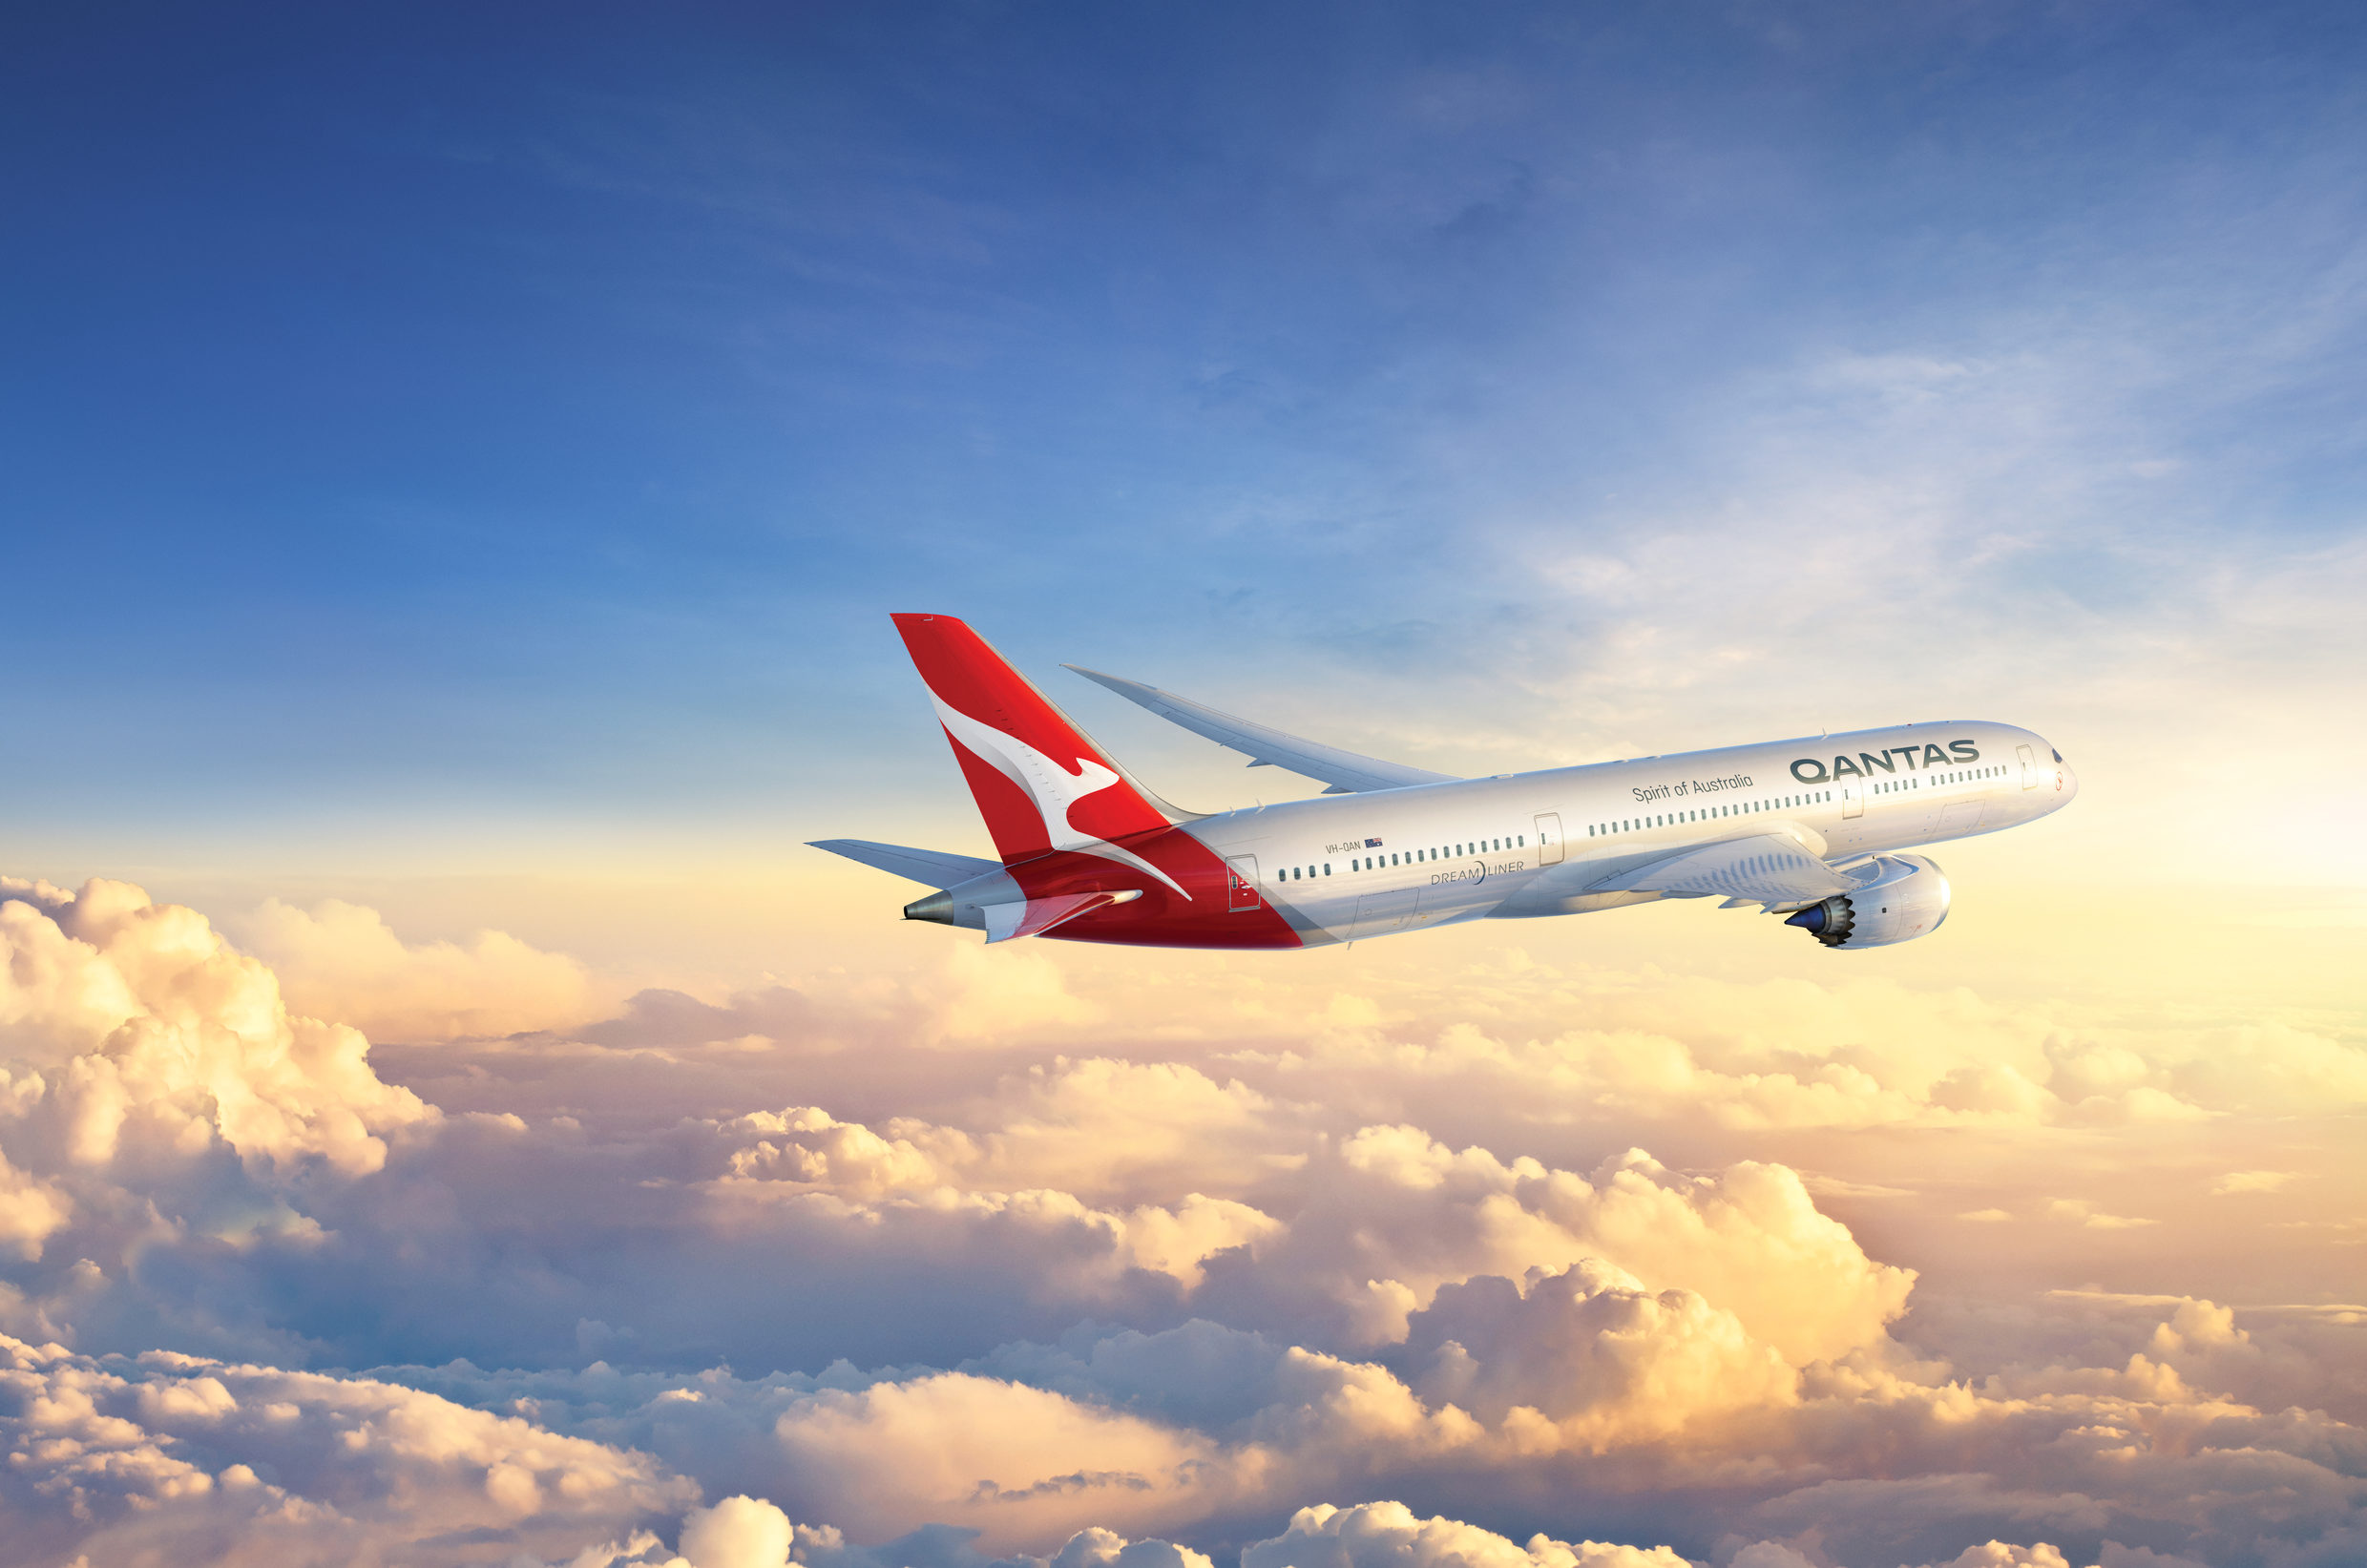
\includegraphics[width=1\textwidth,height=\textheight]{source/figures/full_caption_example.jpg}
\caption{This is not a boat}\label{fig:other_fig}
}
\end{figure}

\chapter{Untersuchung mit Tabelle}\label{sec:research-table}

\section{Einleitung}\label{einleitung-3}

Das ist die Einleitung. Sed vulputate tortor at nisl blandit interdum.
Cras sagittis massa ex, quis eleifend purus condimentum congue. Maecenas
tristique, justo vitae efficitur mollis, mi nulla varius elit, in
consequat ligula nulla ut augue. Phasellus diam sapien, placerat sit
amet tempor non, lobortis tempus ante.

\section{Methode}\label{methode-2}

Donec imperdiet, lectus vestibulum sagittis tempus, turpis dolor euismod
justo, vel tempus neque libero sit amet tortor. Nam cursus commodo
tincidunt.

\subsection{Unterabschnitt 1}\label{unterabschnitt-1-1}

Das ist der erste Teil der Methodik. Duis tempor sapien sed tellus
ultrices blandit. Sed porta mauris tortor, eu vulputate arcu dapibus ac.
Curabitur sodales at felis efficitur sollicitudin. Quisque at neque
sollicitudin, mollis arcu vitae, faucibus tellus.

\subsection{Unterabschnitt 2}\label{unterabschnitt-2-2}

Das ist der zweite Teil der Methodik. Sed ut ipsum ultrices, interdum
ipsum vel, lobortis diam. Curabitur sit amet massa quis tortor molestie
dapibus a at libero. Mauris mollis magna quis ante vulputate consequat.
Integer leo turpis, suscipit ac venenatis pellentesque, efficitur non
sem. Pellentesque eget vulputate turpis. Etiam id nibh at elit fermentum
interdum.

\section{Ergebnisse}\label{ergebnisse-2}

Die Tabelle \ref{tbl:random} zeigt uns wie man eine Tabelle hinzufügt.
Integer tincidunt sed nisl eget pellentesque. Mauris eleifend, nisl non
lobortis fringilla, sapien eros aliquet orci, vitae pretium massa neque
eu turpis. Pellentesque tincidunt aliquet volutpat. Ut ornare dui id ex
sodales laoreet.

\newpage

\def\pandoctableshortcapt{Table short caption}

\hypertarget{tbl:random}{}
\begin{longtable}[]{@{}
  >{\raggedright\arraybackslash}p{(\columnwidth - 4\tabcolsep) * \real{0.2778}}
  >{\raggedright\arraybackslash}p{(\columnwidth - 4\tabcolsep) * \real{0.3333}}
  >{\raggedright\arraybackslash}p{(\columnwidth - 4\tabcolsep) * \real{0.2778}}@{}}
\caption[Table short caption]{\label{tbl:random}Das ist die
Tabellenbeschriftung.}\tabularnewline
\toprule\noalign{}
\begin{minipage}[b]{\linewidth}\raggedright
Spalte 1
\end{minipage} & \begin{minipage}[b]{\linewidth}\raggedright
Spalte 2
\end{minipage} & \begin{minipage}[b]{\linewidth}\raggedright
Spalte 3
\end{minipage} \\
\midrule\noalign{}
\endfirsthead
\toprule\noalign{}
\begin{minipage}[b]{\linewidth}\raggedright
Spalte 1
\end{minipage} & \begin{minipage}[b]{\linewidth}\raggedright
Spalte 2
\end{minipage} & \begin{minipage}[b]{\linewidth}\raggedright
Spalte 3
\end{minipage} \\
\midrule\noalign{}
\endhead
\bottomrule\noalign{}
\endlastfoot
Zeile 1 & 0.1 & 0.2 \\
Zeile 2 & 0.3 & 0.3 \\
Zeile 3 & 0.4 & 0.4 \\
Zeile 4 & 0.5 & 0.6 \\
\end{longtable}

\let\pandoctableshortcapt\relax

\section{Auseinandersetzung}\label{auseinandersetzung-2}

Das ist die Auseinandersetzung mit den Ergebnissen. As we saw in
Table~\ref{tbl:random}, many things are true, and other things are not.
Etiam sit amet mi eros. Donec vel nisi sed purus gravida fermentum at
quis odio. Vestibulum quis nisl sit amet justo maximus molestie.
Maecenas vitae arcu erat. Nulla facilisi. Nam pretium mauris eu enim
porttitor, a mattis velit dictum. Nulla sit amet ligula non mauris
volutpat fermentum quis vitae sapien.

\section{Schlussfolgerung}\label{schlussfolgerung-2}

Das ist die Schlussfolgerung des Kapitels. Nullam porta tortor id
vehicula interdum. Quisque pharetra, neque ut accumsan suscipit, orci
orci commodo tortor, ac finibus est turpis eget justo. Cras sodales nibh
nec mauris laoreet iaculis. Morbi volutpat orci felis, id condimentum
nulla suscipit eu. Fusce in turpis quis ligula tempus scelerisque eget
quis odio. Vestibulum et dolor id erat lobortis ullamcorper quis at sem.

\chapter{Finale Untersuchung}\label{sec:research-final}

\section{Einleitung}\label{einleitung-4}

Das ist die Einleitung. Sed vulputate tortor at nisl blandit interdum.
Cras sagittis massa ex, quis eleifend purus condimentum congue. Maecenas
tristique, justo vitae efficitur mollis, mi nulla varius elit, in
consequat ligula nulla ut augue. Phasellus diam sapien, placerat sit
amet tempor non, lobortis tempus ante.

\section{Methode}\label{methode-3}

Donec imperdiet, lectus vestibulum sagittis tempus, turpis dolor euismod
justo, vel tempus neque libero sit amet tortor. Nam cursus commodo
tincidunt.

\subsection{Unterabschnitt 1}\label{unterabschnitt-1-2}

Das ist der erste Teil der Methodik. Duis tempor sapien sed tellus
ultrices blandit. Sed porta mauris tortor, eu vulputate arcu dapibus ac.
Curabitur sodales at felis efficitur sollicitudin. Quisque at neque
sollicitudin, mollis arcu vitae, faucibus tellus.

\subsection{Unterabschnitt 2}\label{unterabschnitt-2-3}

Das ist der zweite Teil der Methodik. Sed ut ipsum ultrices, interdum
ipsum vel, lobortis diam. Curabitur sit amet massa quis tortor molestie
dapibus a at libero. Mauris mollis magna quis ante vulputate consequat.
Integer leo turpis, suscipit ac venenatis pellentesque, efficitur non
sem. Pellentesque eget vulputate turpis. Etiam id nibh at elit fermentum
interdum.

\section{Ergebnisse}\label{ergebnisse-3}

Das sind die Ergebnisse. In vitae odio at libero elementum fermentum vel
iaculis enim. Nullam finibus sapien in congue condimentum. Curabitur et
ligula et ipsum mollis fringilla.

\section{Auseinandersetzung}\label{auseinandersetzung-3}

Das ist die Auseinandersetzung mit den Ergebnissen. Curabitur gravida
nisl id gravida congue. Duis est nisi, sagittis eget accumsan
ullamcorper, semper quis turpis. Mauris ultricies diam metus,
sollicitudin ultricies turpis lobortis vitae. Ut egestas vehicula enim,
porta molestie neque consectetur placerat. Integer iaculis sapien dolor,
non porta nibh condimentum ut.

\section{Schlussfolgerung}\label{schlussfolgerung-3}

Das ist die Schlussfolgerung des Kapitels. Nulla sed condimentum lectus.
Duis sed tempor erat, at cursus lacus. Nam vitae tempus arcu, id
vestibulum sapien. Cum sociis natoque penatibus et magnis dis parturient
montes, nascetur ridiculus mus.

\chapter{Fazit}\label{sec:conclusion}

\section{Zusammenfassung der Arbeit}\label{zusammenfassung-der-arbeit}

Zusammenfassend pellentesque habitant morbi tristique senectus et netus
et malesuada fames ac turpis egestas. Nunc eleifend, ex a luctus
porttitor, felis ex suscipit tellus, ut sollicitudin sapien purus in
libero. Nulla blandit eget urna vel tempus. Praesent fringilla dui
sapien, sit amet egestas leo sollicitudin at.

\section{Zukünftige Arbeit}\label{zukuxfcnftige-arbeit}

Es gibt mehrere mögliche Richtungen, um diese Arbeit zu erweitern. Lorem
ipsum dolor sit amet, consectetur adipiscing elit. Aliquam gravida ipsum
at tempor tincidunt. Aliquam ligula nisl, blandit et dui eu, eleifend
tempus nibh. Nullam eleifend sapien eget ante hendrerit commodo.
Pellentesque pharetra erat sit amet dapibus scelerisque.

Vestibulum suscipit tellus risus, faucibus vulputate orci lobortis eget.
Nunc varius sem nisi. Nunc tempor magna sapien, euismod blandit elit
pharetra sed. In dapibus magna convallis lectus sodales, a consequat sem
euismod. Curabitur in interdum purus. Integer ultrices laoreet aliquet.
Nulla vel dapibus urna. Nunc efficitur erat ac nisi auctor sodales.

\chapter*{Anhang 1: Einige Extras}\label{anhang-1-einige-extras}
\addcontentsline{toc}{chapter}{Anhang 1: Einige Extras}

\rhead{ANHANG 1}

Füge Anhang 1 hier hinzu. Vivamus hendrerit rhoncus interdum. Sed
ullamcorper et augue at porta. Suspendisse facilisis imperdiet urna, eu
pellentesque purus suscipit in. Integer dignissim mattis ex aliquam
blandit. Curabitur lobortis quam varius turpis ultrices egestas.

\chapter*{Anhang 2: Noch mehr Extras}\label{anhang-2-noch-mehr-extras}
\addcontentsline{toc}{chapter}{Anhang 2: Noch mehr Extras}

\rhead{ANHANG 2}

Füge Anhang 2 hier hinzu. Aliquam rhoncus mauris ac neque imperdiet, in
mattis eros aliquam. Etiam sed massa et risus posuere rutrum vel et
mauris. Integer id mauris sed arcu venenatis finibus. Etiam nec
hendrerit purus, sed cursus nunc. Pellentesque ac luctus magna. Aenean
non posuere enim, nec hendrerit lacus. Etiam lacinia facilisis tempor.
Aenean dictum nunc id felis rhoncus aliquam.

\footnotesize
\singlespacing
\setlength{\parindent}{0in}

\chapter{Literaturverzeichnis}\label{literaturverzeichnis}

\rhead{LITERATURVERZEICHNIS}

\hypertarget{refs}{}
\begin{CSLReferences}{0}{0}
\leavevmode\vadjust pre{\hypertarget{ref-phd_thesis_markdown}{}}%
\CSLLeftMargin{{[}1{]} }%
\CSLRightInline{Tom Pollard; Marvin Reimer; David San; Arco Mul; Matthew
Gwynfryn Thomas; Jakub Nowosad; Dennis Weissmann; W. Caleb McDaniel.
2016. \emph{Template for writing a PhD thesis in Markdown}. Tom Pollard.
Abgerufen 1. November 2017 von
\url{https://github.com/tompollard/phd_thesis_markdown/tree/v1.0}}

\end{CSLReferences}

\end{document}
